\section{Systemabgrenzung}
\label{sec:systemabgrenzung}

\subsection{Systemkontext}

Im Kontextdiagramm (Abbildung \ref{fig:systemkontext}) sind alle für die
folgenden Betrachtungen relevanten Umsysteme aufgezeigt. Die Verbindungslinien
zeigen die Kommunikation zu/von unserem System, ohne dabei auf Inhalt oder
Richtung einzugehen.
\\[\intextsep]
\begin{minipage}{\linewidth}
\centering%
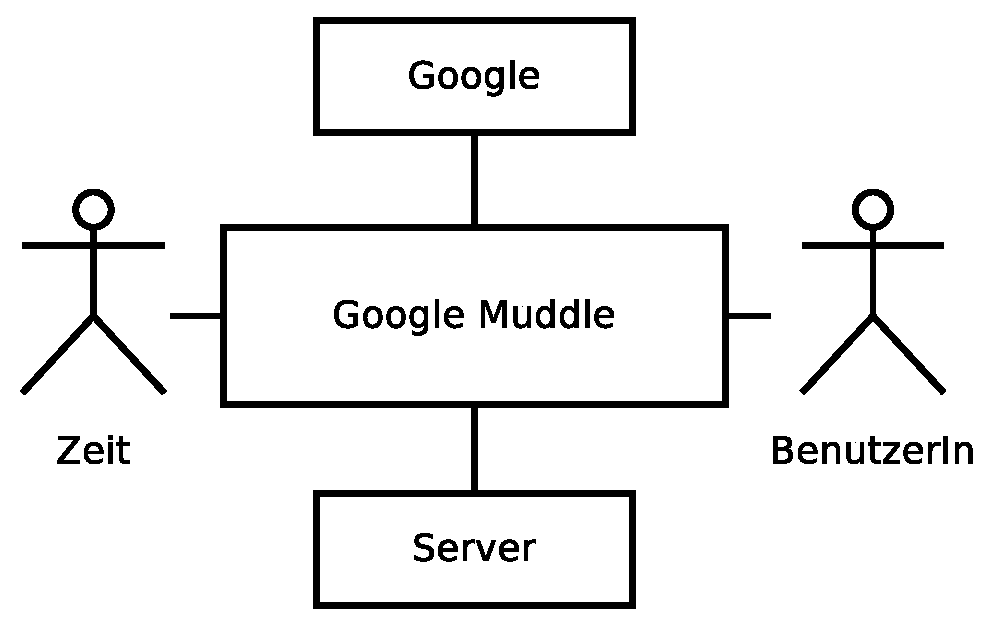
\includegraphics[scale=0.4,clip=]{img/systemkontext.eps}%
\figcaption{Systemkontext \textit{Google Muddle}}%
\label{fig:systemkontext}%
\end{minipage}

\subsection{AkteurInnen}

\subsubsection*{Zeit}

Die Zeit kann zu festgelegten Zeiten oder in bestimmten Intervallen
Anwendungsfälle auslösen.

\subsubsection*{BenutzerIn}

Mit BenutzerIn ist die Person gemeint, welche einen Browser mit \textit{Google
Muddle} als Erweiterung verwendet. Der/die BenutzerIn gilt als AkteurIn,
interagiert aber nur indirekt (über den Browser) mit dem System \textit{Google
Muddle}.

\subsection{Umsysteme}

\subsubsection*{Google}

Anwendungsfälle werden mit der Suchmaschine von Google interagieren.

\subsubsection*{Server}

Die Server-Komponente von \textit{Google Muddle}, welche hier (im Rahmen dieser
Modularbeit) nicht spezifiziert wird, wird ebenfalls mit der Applikation
interagieren.
